\documentclass[12pt]{article}
\usepackage[table]{xcolor}
\usepackage[shortlabels]{enumitem}
\usepackage{tabularx,xltabular}
\usepackage{graphicx}
\usepackage{hyperref}
\usepackage{verbatim}
\usepackage{geometry}
\usepackage{ulem}
\usepackage[official]{eurosym}
\usepackage{tikz}
\usetikzlibrary{arrows,backgrounds,calc,decorations.markings,patterns,3d}
\usepackage{pgfplots}
\pgfplotsset{compat = newest}
\usetikzlibrary{fit}
\newcommand\addvmargin[1]{
\usetikzlibrary{arrows}
\node[fit=(current bounding box),inner ysep=#1,inner xsep=0]{};}
\usepackage{cancel}
\usepackage{fontspec}
\usepackage{array}  
\geometry{a4paper, top=2cm, left=2cm, right=2cm, bottom=2cm, headsep=1cm}
\usepackage{tabu}
\usepackage{pst-node}
\usepackage{colortbl}
\usepackage{array}
\usepackage{german}
\setlength\parindent{0pt}
\newcolumntype{?}{!{\vrule width 1pt}}
\usepackage{makecell}
\renewcommand{\arraystretch}{2.5}
\usepackage{pbox}
\usepackage{amssymb}
\usepackage{amsmath}
\usepackage{booktabs}
\newcolumntype{L}[1]{>{\raggedright\let\newline\\\arraybackslash\hspace{0pt}}m{#1}}
\newcolumntype{C}[1]{>{\centering\let\newline\\\arraybackslash\hspace{0pt}}m{#1}}
\newcolumntype{R}[1]{>{\raggedleft\let\newline\\\arraybackslash\hspace{0pt}}m{#1}}
\begin{document}
\rightline{Datum: 14.06.2023}
\centerline{{\Large Tägliche Übungen}} 
\vspace{1cm}
\noindent \\


\begin{xltabular}{\textwidth}{|C{0.75cm}|X|}
\arrayrulecolor{black}\hline
a)&Berechne die Variable $$46=y-27$$
\\\hline
b)&Berechne die Variable $$28=a+6$$
\\\hline
c)&Berechne die Variable $$36=b+33$$
\\\hline
d)&Berechne die Variable $$36=y-10$$
\\\hline
e)&Berechne die Variable $$44=b-43$$
\\\hline
f)&Berechne die Variable $$19=y+30$$
\\\hline
g)&Berechne die Variable $$-3+2\cdot y-14+5\cdot y=11$$
\\\hline
h)&Berechne die Variable $$5\cdot y-3+4\cdot y-10=50$$
\\\hline
i)&Berechne die Variable $$1\cdot y-4-3+7\cdot y=9$$
\\\hline
\end{xltabular}
\vspace{0.5cm}
\newpage
\rightline{Datum: 14.06.2023}
\centerline{{\large Lösungen Tägliche Übungen}} 
\vspace{0.5cm}

\begin{xltabular}{\textwidth}{|C{0.75cm}|X|}
\arrayrulecolor{black}\hline
a)&\begingroup\setlength{\jot}{-0.03cm}
\tikzstyle{background grid}=[draw, black!15,step=.5cm]
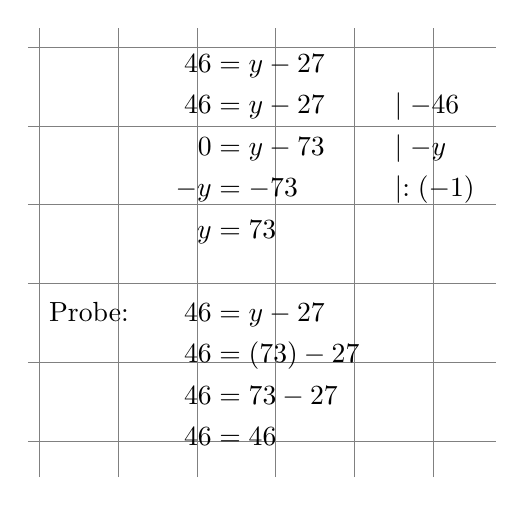
\begin{tikzpicture}[show background grid]
\node[below right] at (0,0.1) {
$\begin{aligned}
46 &=y-27& &  \\
46 &=y - 27& & \mid -46\\
0 &=y - 73& & \mid -y \\
-y &=-73& & \mid :\left(-1\right)\\
y &=73& & 
\\
\\
\mbox{Probe:}\qquad 46 &=y-27& &  \\
46 &=\left(73\right)-27& &  \\
46 &=73-27& &  \\
46 &=46& &  \\
\end{aligned}$};
\end{tikzpicture}
\endgroup
\\\hline
b)&\begingroup\setlength{\jot}{-0.03cm}
\tikzstyle{background grid}=[draw, black!15,step=.5cm]
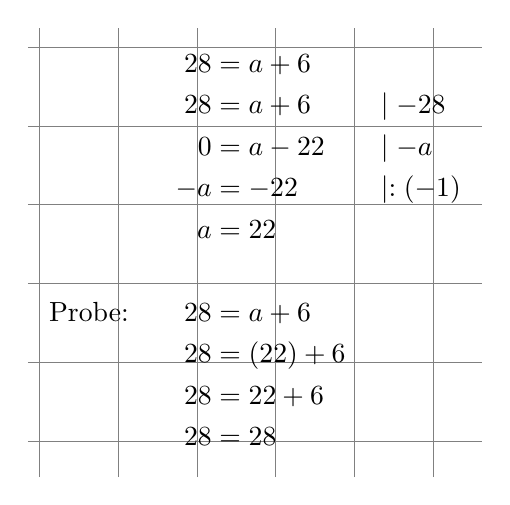
\begin{tikzpicture}[show background grid]
\node[below right] at (0,0.1) {
$\begin{aligned}
28 &=a+6& &  \\
28 &=a + 6& & \mid -28\\
0 &=a - 22& & \mid -a \\
-a &=-22& & \mid :\left(-1\right)\\
a &=22& & 
\\
\\
\mbox{Probe:}\qquad 28 &=a+6& &  \\
28 &=\left(22\right)+6& &  \\
28 &=22+6& &  \\
28 &=28& &  \\
\end{aligned}$};
\end{tikzpicture}
\endgroup
\\\hline
c)&\begingroup\setlength{\jot}{-0.03cm}
\tikzstyle{background grid}=[draw, black!15,step=.5cm]
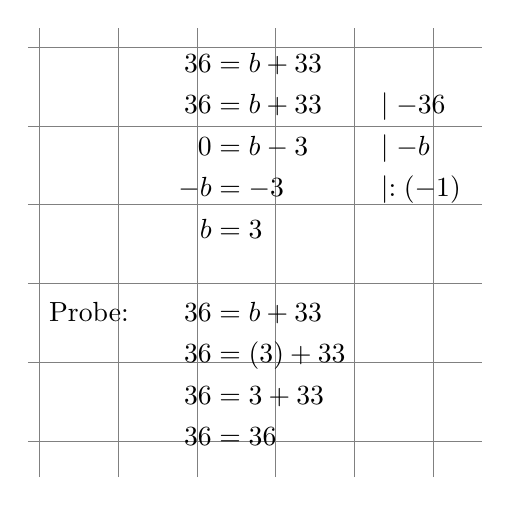
\begin{tikzpicture}[show background grid]
\node[below right] at (0,0.1) {
$\begin{aligned}
36 &=b+33& &  \\
36 &=b + 33& & \mid -36\\
0 &=b - 3& & \mid -b \\
-b &=-3& & \mid :\left(-1\right)\\
b &=3& & 
\\
\\
\mbox{Probe:}\qquad 36 &=b+33& &  \\
36 &=\left(3\right)+33& &  \\
36 &=3+33& &  \\
36 &=36& &  \\
\end{aligned}$};
\end{tikzpicture}
\endgroup
\\\hline
d)&\begingroup\setlength{\jot}{-0.03cm}
\tikzstyle{background grid}=[draw, black!15,step=.5cm]
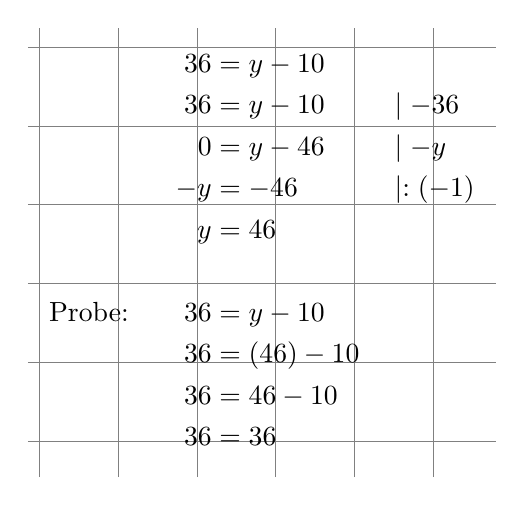
\begin{tikzpicture}[show background grid]
\node[below right] at (0,0.1) {
$\begin{aligned}
36 &=y-10& &  \\
36 &=y - 10& & \mid -36\\
0 &=y - 46& & \mid -y \\
-y &=-46& & \mid :\left(-1\right)\\
y &=46& & 
\\
\\
\mbox{Probe:}\qquad 36 &=y-10& &  \\
36 &=\left(46\right)-10& &  \\
36 &=46-10& &  \\
36 &=36& &  \\
\end{aligned}$};
\end{tikzpicture}
\endgroup
\\\hline
e)&\begingroup\setlength{\jot}{-0.03cm}
\tikzstyle{background grid}=[draw, black!15,step=.5cm]
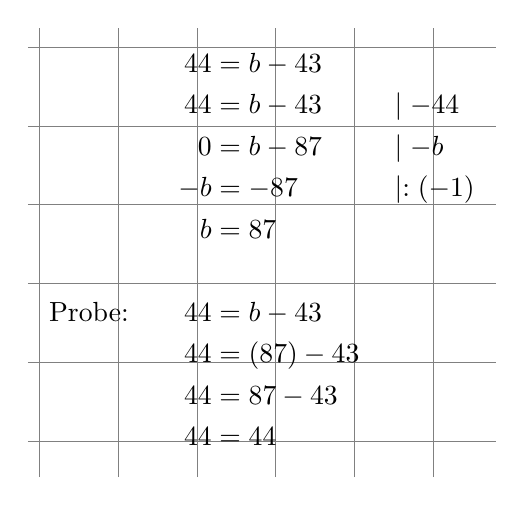
\begin{tikzpicture}[show background grid]
\node[below right] at (0,0.1) {
$\begin{aligned}
44 &=b-43& &  \\
44 &=b - 43& & \mid -44\\
0 &=b - 87& & \mid -b \\
-b &=-87& & \mid :\left(-1\right)\\
b &=87& & 
\\
\\
\mbox{Probe:}\qquad 44 &=b-43& &  \\
44 &=\left(87\right)-43& &  \\
44 &=87-43& &  \\
44 &=44& &  \\
\end{aligned}$};
\end{tikzpicture}
\endgroup
\\\hline
f)&\begingroup\setlength{\jot}{-0.03cm}
\tikzstyle{background grid}=[draw, black!15,step=.5cm]
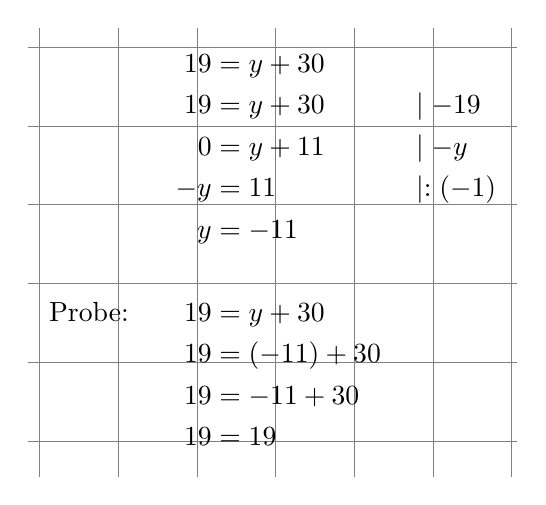
\begin{tikzpicture}[show background grid]
\node[below right] at (0,0.1) {
$\begin{aligned}
19 &=y+30& &  \\
19 &=y + 30& & \mid -19\\
0 &=y + 11& & \mid -y \\
-y &=11& & \mid :\left(-1\right)\\
y &=-11& & 
\\
\\
\mbox{Probe:}\qquad 19 &=y+30& &  \\
19 &=\left(-11\right)+30& &  \\
19 &=-11+30& &  \\
19 &=19& &  \\
\end{aligned}$};
\end{tikzpicture}
\endgroup
\\\hline
g)&\begingroup\setlength{\jot}{-0.03cm}
\tikzstyle{background grid}=[draw, black!15,step=.5cm]
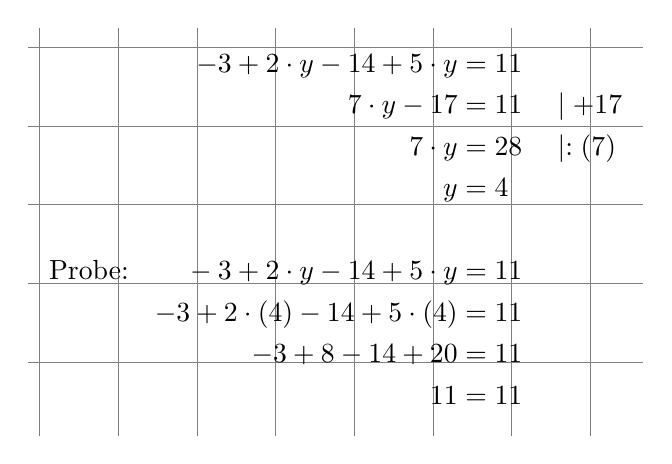
\begin{tikzpicture}[show background grid]
\node[below right] at (0,0.1) {
$\begin{aligned}
-3+2\cdot y-14+5\cdot y &=11& &  \\
7\cdot y - 17 &=11& & \mid + 17\\
7\cdot y &=28& & \mid :\left(7\right)\\
y &=4& & 
\\
\\
\mbox{Probe:}\qquad -3+2\cdot y-14+5\cdot y &=11& &  \\
-3+2\cdot \left(4\right)-14+5\cdot \left(4\right) &=11& &  \\
-3+8-14+20 &=11& &  \\
11 &=11& &  \\
\end{aligned}$};
\end{tikzpicture}
\endgroup
\\\hline
h)&\begingroup\setlength{\jot}{-0.03cm}
\tikzstyle{background grid}=[draw, black!15,step=.5cm]
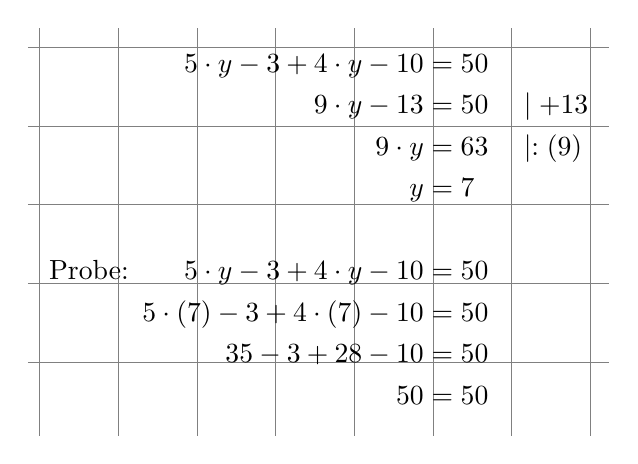
\begin{tikzpicture}[show background grid]
\node[below right] at (0,0.1) {
$\begin{aligned}
5\cdot y-3+4\cdot y-10 &=50& &  \\
9\cdot y - 13 &=50& & \mid + 13\\
9\cdot y &=63& & \mid :\left(9\right)\\
y &=7& & 
\\
\\
\mbox{Probe:}\qquad 5\cdot y-3+4\cdot y-10 &=50& &  \\
5\cdot \left(7\right)-3+4\cdot \left(7\right)-10 &=50& &  \\
35-3+28-10 &=50& &  \\
50 &=50& &  \\
\end{aligned}$};
\end{tikzpicture}
\endgroup
\\\hline
i)&\begingroup\setlength{\jot}{-0.03cm}
\tikzstyle{background grid}=[draw, black!15,step=.5cm]
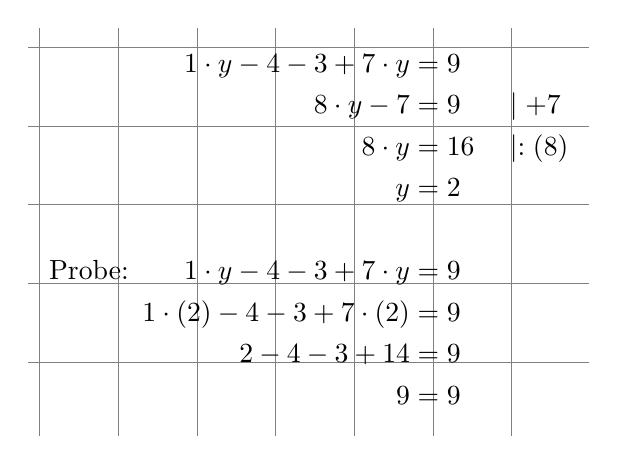
\begin{tikzpicture}[show background grid]
\node[below right] at (0,0.1) {
$\begin{aligned}
1\cdot y-4-3+7\cdot y &=9& &  \\
8\cdot y - 7 &=9& & \mid + 7\\
8\cdot y &=16& & \mid :\left(8\right)\\
y &=2& & 
\\
\\
\mbox{Probe:}\qquad 1\cdot y-4-3+7\cdot y &=9& &  \\
1\cdot \left(2\right)-4-3+7\cdot \left(2\right) &=9& &  \\
2-4-3+14 &=9& &  \\
9 &=9& &  \\
\end{aligned}$};
\end{tikzpicture}
\endgroup
\\\hline
\end{xltabular}
\vspace{0.5cm}
\end{document}